\part{Versuch}
\section{Aufbau}
Der Versuchsaufbau wurde im Zimmer 2.001b mit einem Servomotor aus den Praktikas durchgeführt. Er kann zwischen -2500 bis +2500 $\nicefrac{U}{min}$ betrieben werden und im \textit{Syncronisation Mode} auf 1 $\nicefrac{U}{min}$ genau eingestellt werden. Im \textit{Speed-Control Mode} liegt die Schrittweite bei 10 $\nicefrac{U}{min}$.

\begin{figure}[ht]
    \centering
    %    \missingfigure{Bild einfügen}    
    \begin{subfigure}[c]{0.8\textwidth}       
        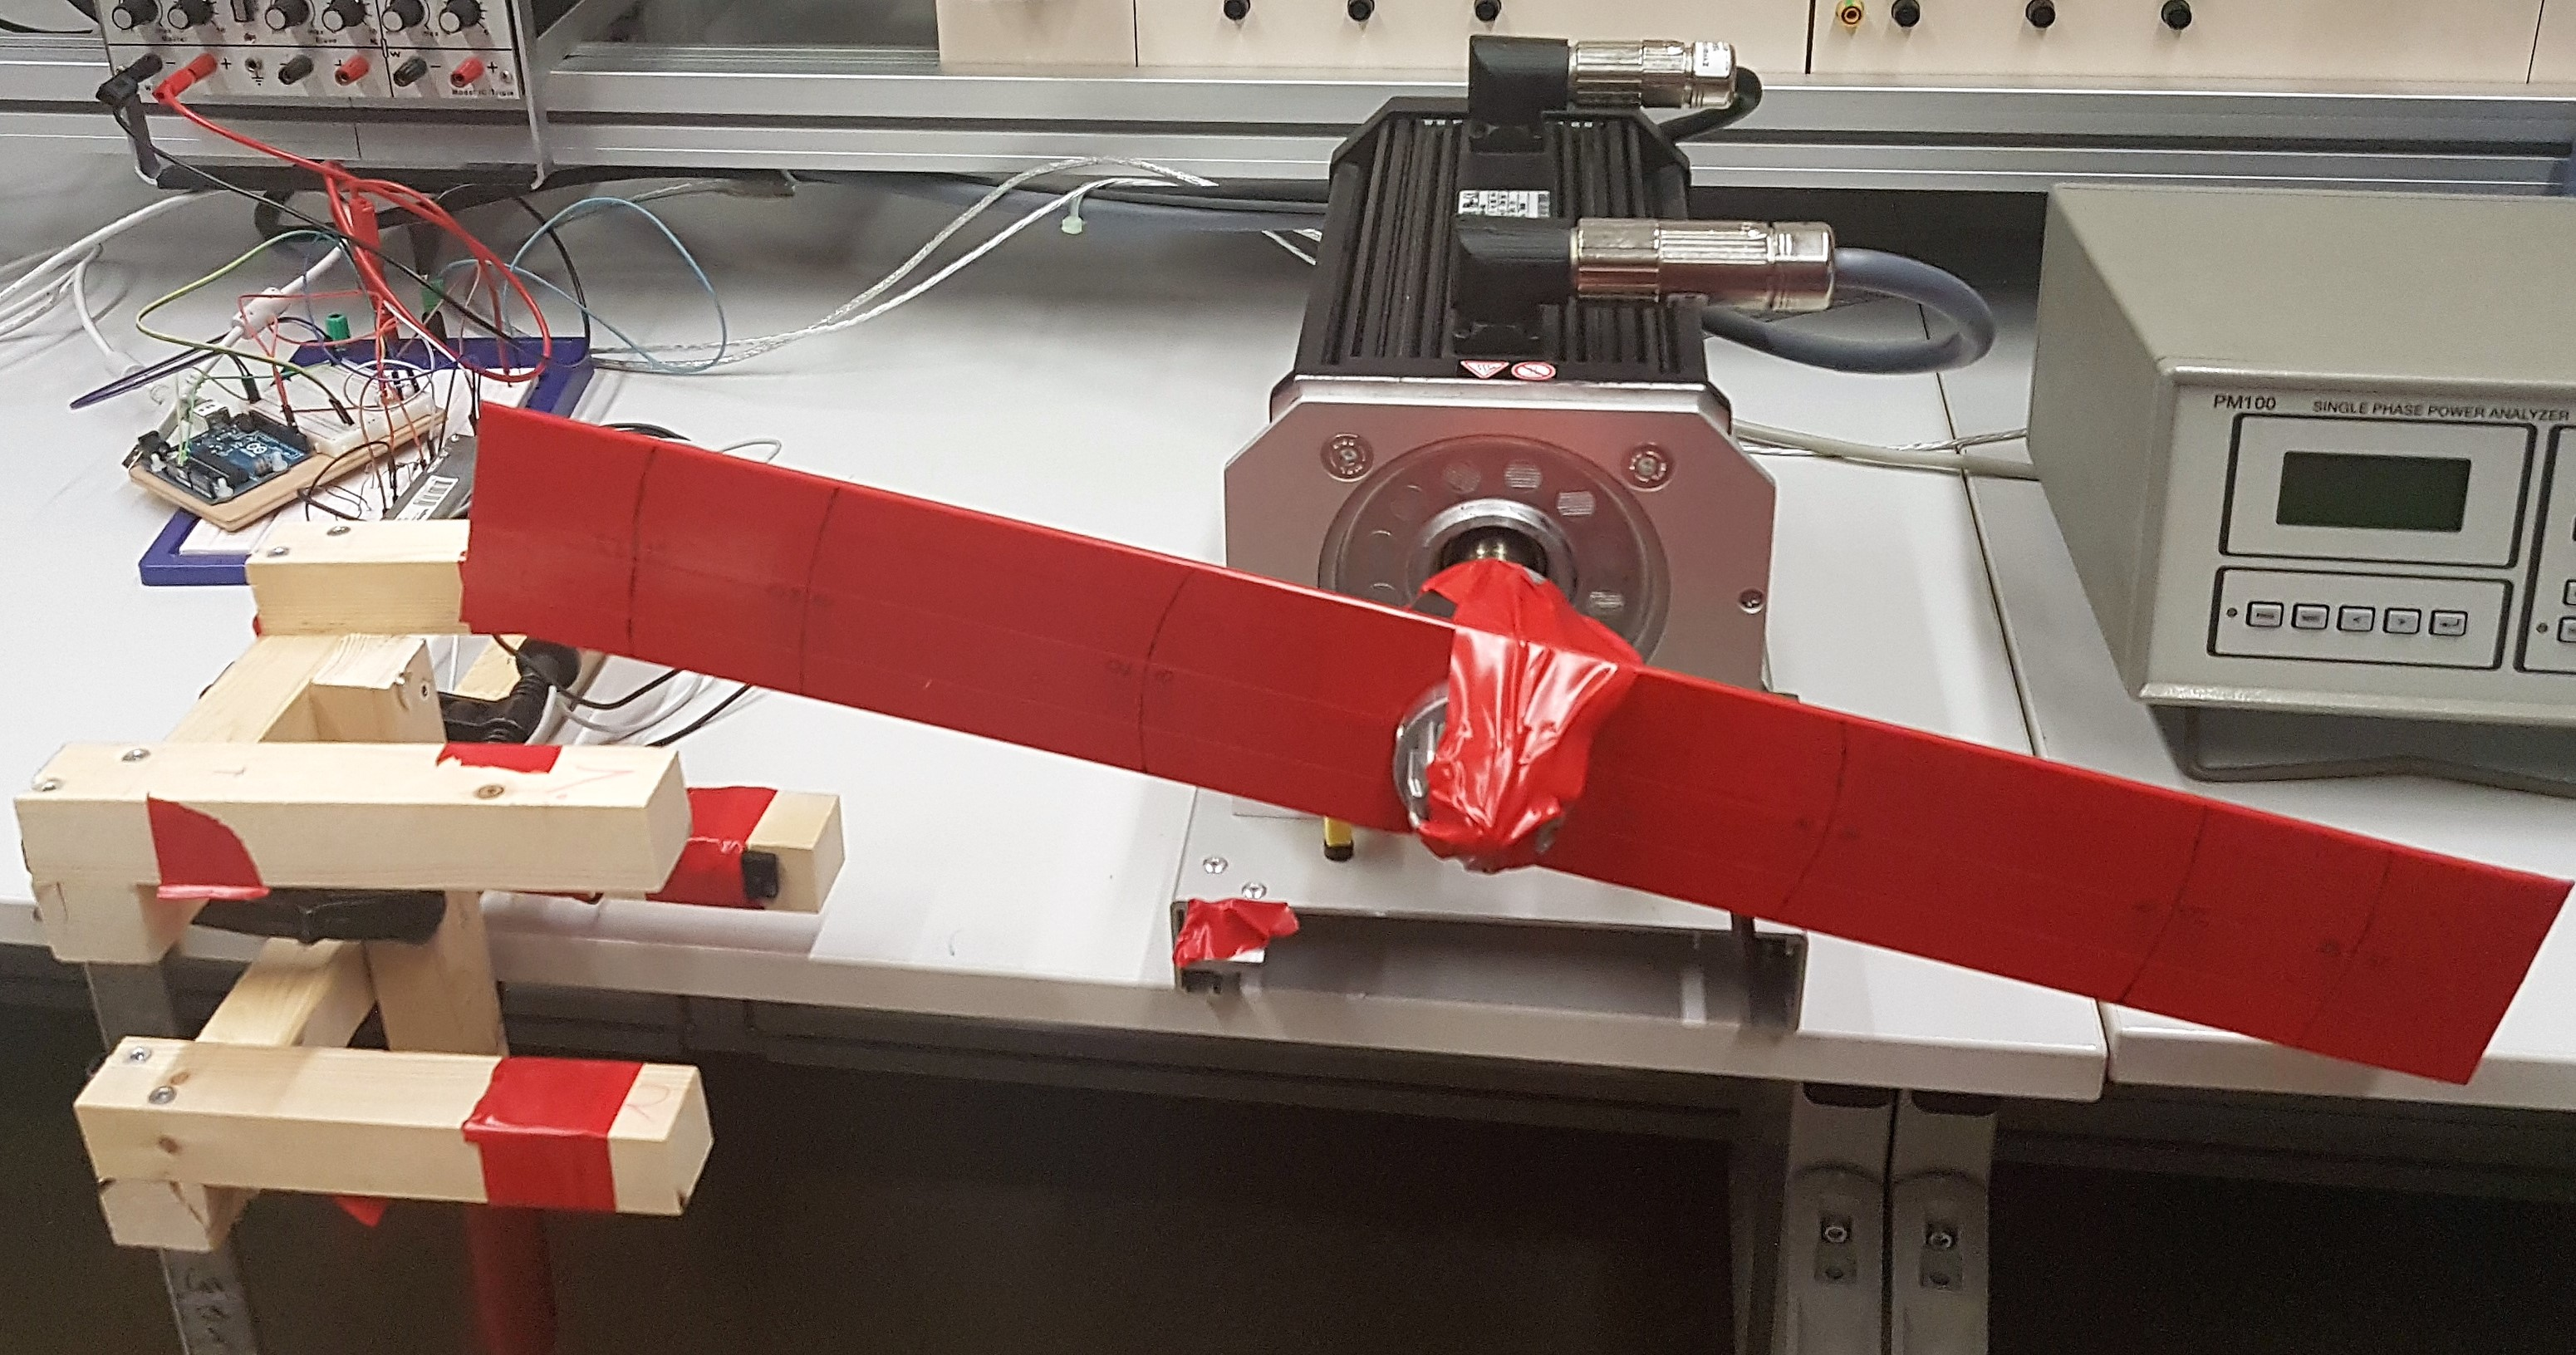
\includegraphics[width=\textwidth]{images/Aufbau.jpg}
        \subcaption{Übersicht}          
    \end{subfigure}

    \begin{subfigure}[c]{0.8\textwidth}
        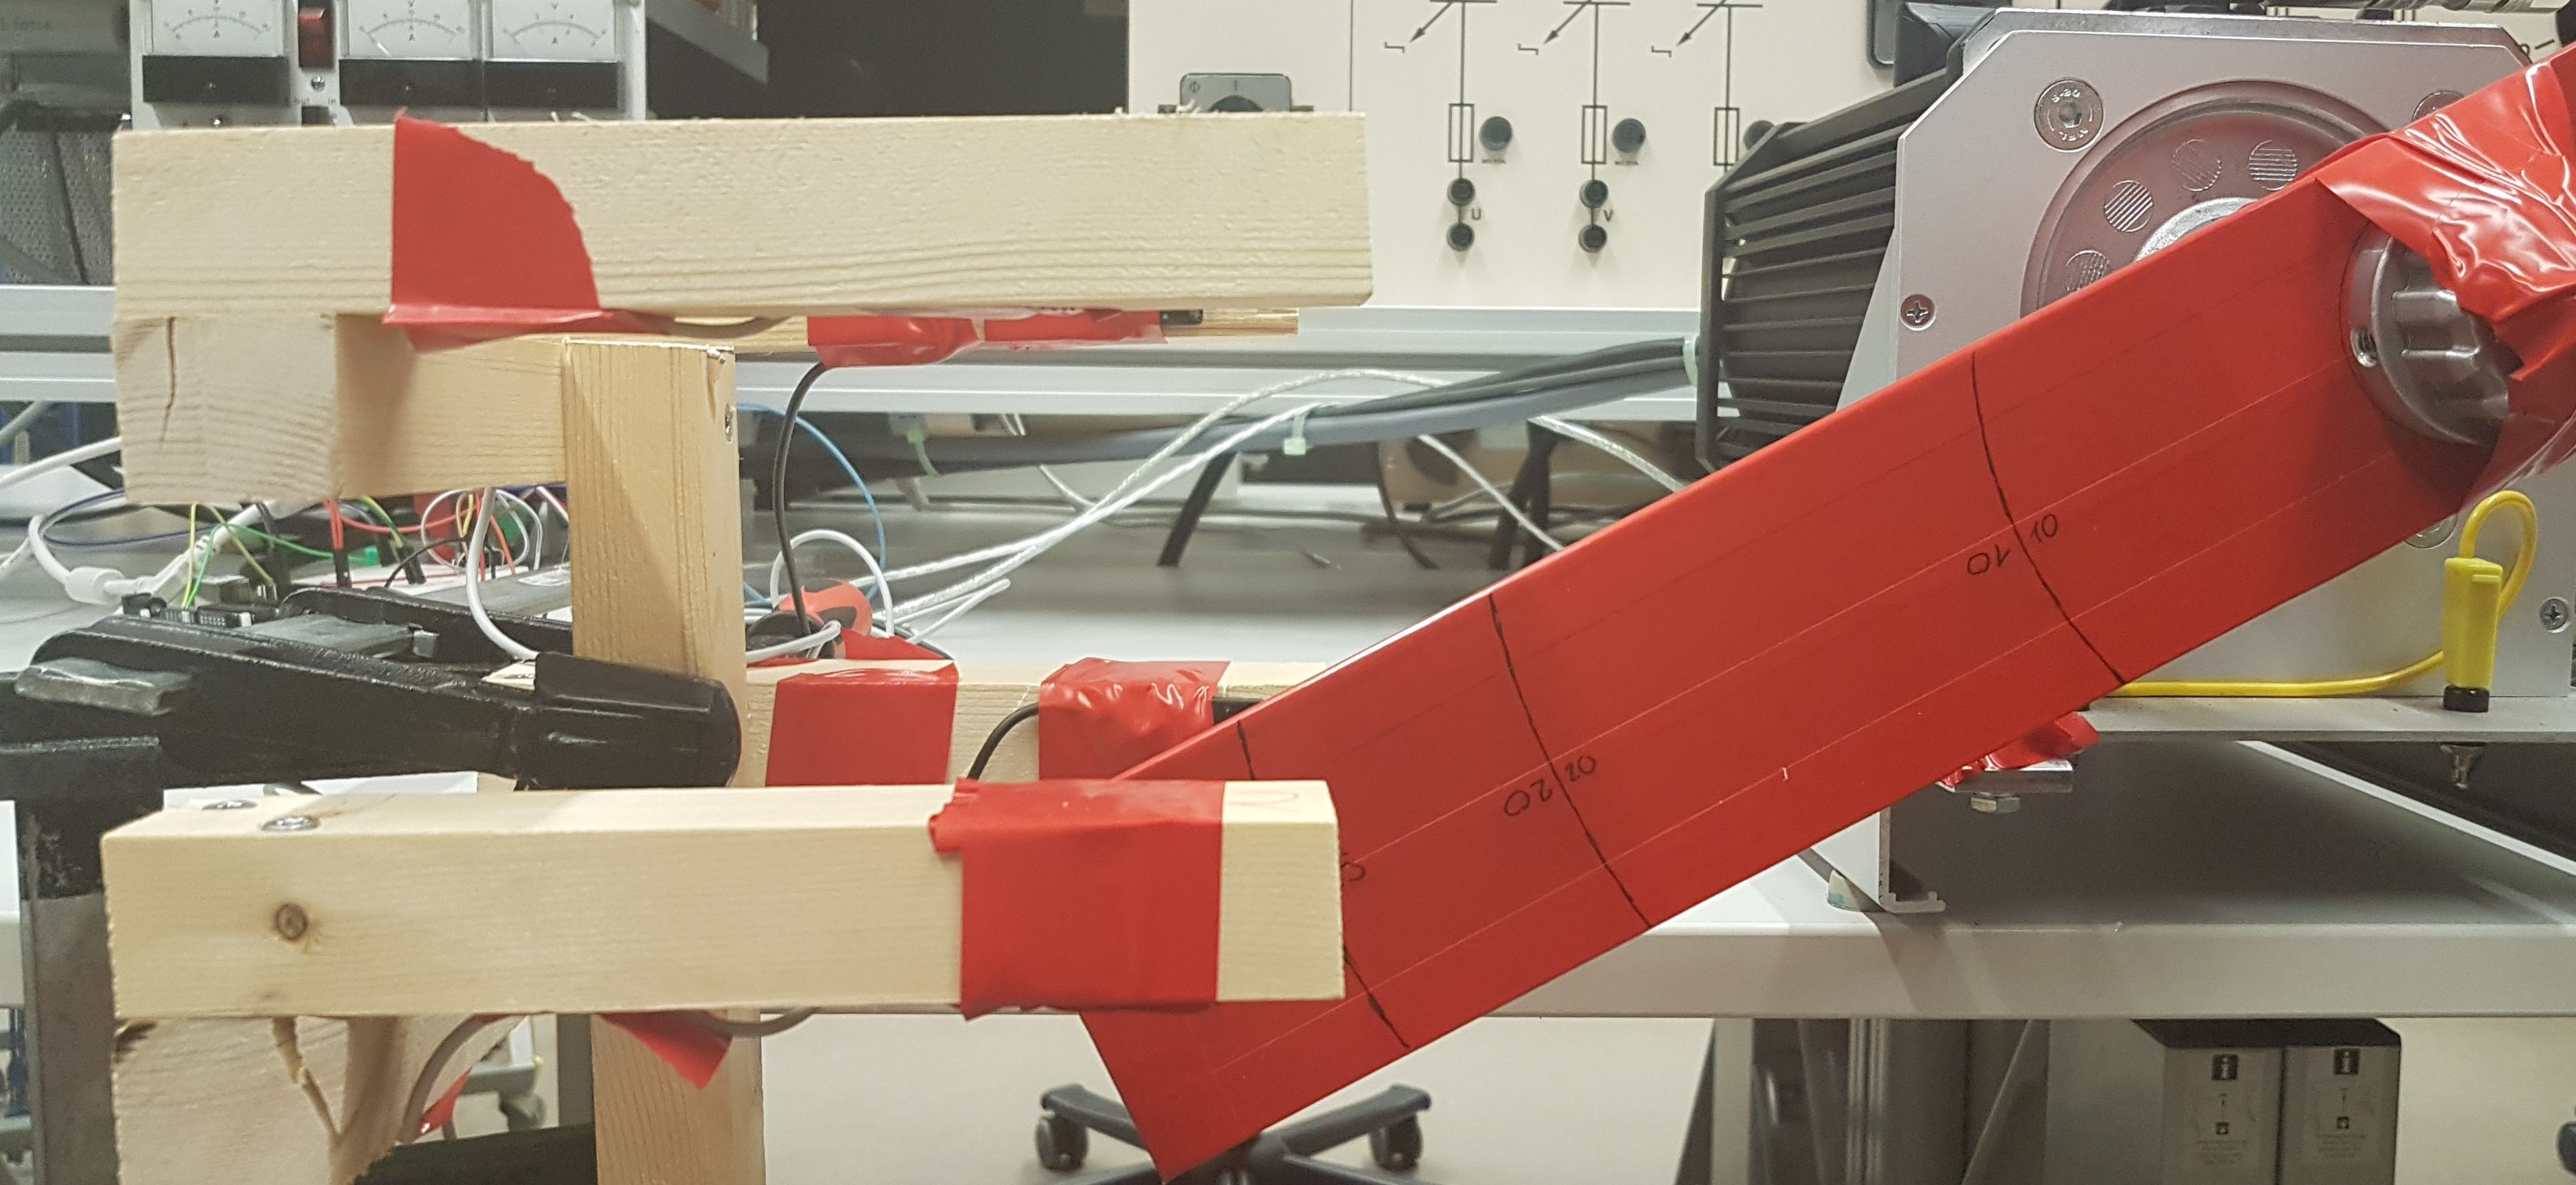
\includegraphics[width=\textwidth]{images/AufbauDetail.jpg}
        \subcaption{Detail}
    \end{subfigure}
    \caption{Versuchsaufbau}\label{fig:Aufbau}   
\end{figure}

Die Lichtschranken wurden mit Hilfe einer Holzkonstruktion montiert.\\
Sie haben einen Abstand von 100 mm.\\
Der \marg{Rotor} Rotor ist 72 mm breit und somit die Dimension eines Unihockeyballs.\\

Bei einem Durchmesser von 50 cm ergibt sich mit 2000 $\nicefrac{U}{min}$ eine Umfangsgeschwindigkeit von 188.5 $\nicefrac{km}{h}$ wie man dem Anhang \ref{app:berechnung} entnehmen kann.